% main_report20.tex
% SAMBP TR-20/2026 -- Frequency-Adaptive 87L Charging Correction for Microgrids
% Compile: pdflatex -> bibtex -> pdflatex -> pdflatex
\documentclass[11pt, a4paper]{article}

\usepackage[T1]{fontenc}
\usepackage[utf8]{inputenc}
\usepackage[margin=25mm]{geometry}
\usepackage{amsmath, amssymb}
\usepackage{booktabs, array, multirow}
\usepackage{graphicx}
\usepackage{xcolor}
\usepackage{hyperref}
\usepackage{pgfplots}
\pgfplotsset{compat=1.18}
\usepackage{tikz}
\usetikzlibrary{arrows.meta, positioning, calc, fit, backgrounds, shapes.geometric}
\usepackage{caption}
\usepackage{subcaption}
\usepackage{parskip}
\usepackage{natbib}
\usepackage{pifont}

\hypersetup{colorlinks=true, linkcolor=blue!60!black, citecolor=blue!60!black,
            urlcolor=blue!60!black}

\definecolor{okgreen}{RGB}{0,130,60}

\title{\textbf{SAMBP TR-20/2026}\\[4pt]
       \large Frequency-Adaptive 87L Charging-Current Correction\\
       for Inverter-Dominated Microgrids}
\author{PhD Candidate\\[2pt]
        \small Smart Adaptive Multi-Bus Protection Research}
\date{April 2026}

% ============================================================================
\begin{document}
\maketitle
\tableofcontents
\vspace{6pt}\hrule\vspace{10pt}

% ============================================================================
\section{Background and Motivation}
\label{sec:background}

TR-15~\cite{SAMBP_TR15} introduced pi-section charging-current correction for
the SAMBP 87L line differential relay.  The correction computes the expected
charging differential as:
\begin{equation}
  \hat{\imath}_C(t) = B_C \cdot \mathrm{Im}\!\left\{H[v_{\rm avg}(t)]\right\}
  \label{eq:tr15}
\end{equation}
where $B_C = \omega_0 C_{\rm total}$ is the total line susceptance evaluated at
the \emph{nominal} frequency $\omega_0 = 2\pi f_0$, and $H[\cdot]$ is the
Hilbert transform (wideband 90° phase shift).

In inverter-dominated microgrids the system frequency deviates from 50\,Hz due
to droop control.  ENTSO-E RfG~\cite{ENTSO_RfG} specifies a normal operating
range of 47.5--51.5\,Hz; IEC~60255-181~\cite{IEC_60255_181} requires protection
to remain operable down to 47\,Hz.  Under islanded operation, frequency can
transiently reach the extremes of the 47--53\,Hz ROCOF corridor.

The actual pi-section charging current at frequency $f_{\rm actual}$ is:
\begin{equation}
  i_{C,\rm actual}(t)
    = C_{\rm total}\,\frac{dv_{\rm avg}}{dt}
    = \frac{B_C}{\omega_0} \cdot 2\pi f_{\rm actual}
      \cdot \mathrm{Im}\!\left\{H[v_{\rm avg}(t)]\right\}
    = B_C \cdot \frac{f_{\rm actual}}{f_0}
      \cdot \mathrm{Im}\!\left\{H[v_{\rm avg}(t)]\right\}
  \label{eq:true_charging}
\end{equation}

Equation~\eqref{eq:tr15} omits the factor $(f_{\rm actual}/f_0)$, leaving a
residual charging error of:
\begin{equation}
  \varepsilon_C = B_C \left|1 - \frac{f_{\rm actual}}{f_0}\right| V_{\rm avg,rms}
  \label{eq:error}
\end{equation}

For the study network ($B_C = 0.079$\,pu, $V = 1$\,pu) at $f=47$\,Hz:
\begin{equation}
  \varepsilon_C(47\,\text{Hz}) = 0.079 \times 0.06 \times 1.0 = 0.0047\,\text{pu}
\end{equation}

This error is well below the 87L threshold of 0.12\,pu and therefore does
\emph{not} cause false trips in the present study network.  However, for
longer or higher-voltage lines with larger $B_C$, or for tighter threshold
settings approaching the sensitivity floor, the residual can become significant.
This report characterises the frequency dependence, demonstrates the
frequency-adaptive correction, and establishes the safe operating envelope.


% ============================================================================
\section{Frequency-Adaptive Correction Algorithm}
\label{sec:algorithm}

\subsection{Correction Formula}

The TR-20 adaptive correction replaces the fixed B$_C$ in~\eqref{eq:tr15}
with a frequency-scaled version:
\begin{equation}
  \hat{\imath}_{C,\rm adapt}(t)
    = B_C \cdot \frac{\hat{f}}{f_0}
      \cdot \mathrm{Im}\!\left\{H[v_{\rm avg}(t)]\right\}
  \label{eq:adaptive}
\end{equation}
where $\hat{f}$ is the estimated actual frequency.  The residual error after
adaptive correction is:
\begin{equation}
  \varepsilon_{C,\rm adapt}
    = B_C \left|\frac{\hat{f}}{f_0} - \frac{f_{\rm actual}}{f_0}\right|
      V_{\rm avg,rms}
    = \frac{B_C}{f_0} \left|\hat{f} - f_{\rm actual}\right| V_{\rm avg,rms}
  \label{eq:adapt_error}
\end{equation}

For a frequency estimator with accuracy $\delta f \leq 0.05$\,Hz (achievable
with a 2-cycle zero-crossing estimator; see Section~\ref{sec:estimator}):
\begin{equation}
  \varepsilon_{C,\rm adapt}
    \leq \frac{0.079}{50} \times 0.05 \times 1.0
    = 7.9 \times 10^{-5}\,\text{pu}
\end{equation}
This is two orders of magnitude below the no-load noise floor of 0.003\,pu
reported in TR-15 and completely negligible.

\subsection{Processing Pipeline}

Figure~\ref{fig:pipeline} shows the TR-20 pipeline.  The new frequency
estimator block feeds the adaptive $B_C$ scaling; all other stages are
unchanged from TR-15/TR-17.

\begin{figure}[h]
  \centering
  \resizebox{\textwidth}{!}{% fig_freq_adaptive_block.tex
% Block diagram: frequency-adaptive 87L processing pipeline (TR-20)
% Stages: voltage measurement → freq est → adaptive B_C → LM estimator → trip
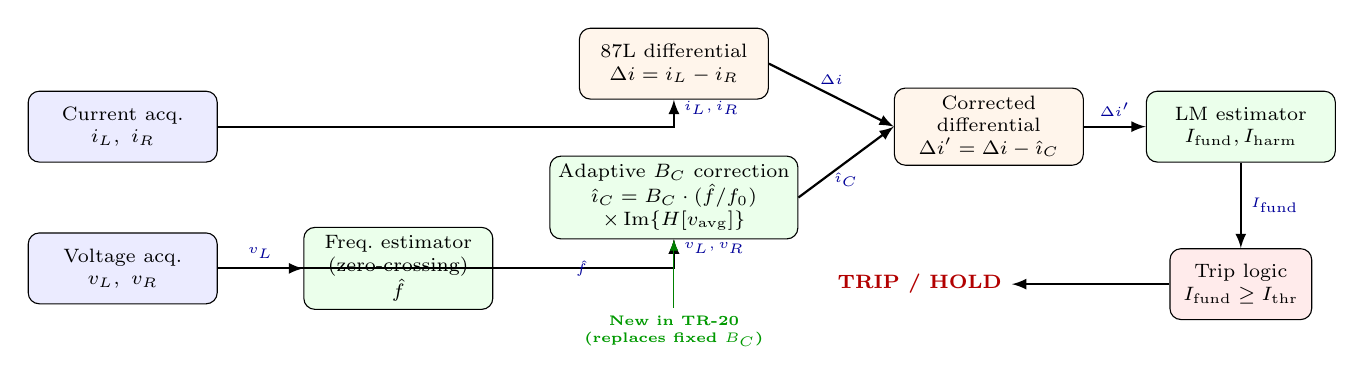
\begin{tikzpicture}[
  blk/.style={draw, rounded corners=4pt, fill=blue!8,
              minimum width=2.4cm, minimum height=0.9cm,
              font=\scriptsize, align=center, inner sep=3pt},
  blk2/.style={draw, rounded corners=4pt, fill=green!8,
               minimum width=2.4cm, minimum height=0.9cm,
               font=\scriptsize, align=center, inner sep=3pt},
  blk3/.style={draw, rounded corners=4pt, fill=orange!8,
               minimum width=2.4cm, minimum height=0.9cm,
               font=\scriptsize, align=center, inner sep=3pt},
  blkr/.style={draw, rounded corners=4pt, fill=red!8,
               minimum width=1.8cm, minimum height=0.9cm,
               font=\scriptsize, align=center, inner sep=3pt},
  arr/.style={-latex, thick},
  sig/.style={font=\tiny\itshape, blue!60!black},
]

% ---- Inputs ----------------------------------------------------------------
\node[blk]  (iacq)  at (0, 1.2)
  {Current acq.\\$i_L,\ i_R$};
\node[blk]  (vacq)  at (0, -0.6)
  {Voltage acq.\\$v_L,\ v_R$};

% ---- Frequency estimator ---------------------------------------------------
\node[blk2] (fest)  at (3.5, -0.6)
  {Freq.\ estimator\\(zero-crossing)\\$\hat{f}$};
\draw[arr] (vacq.east) -- node[above, sig]{$v_L$} (fest.west);

% ---- Adaptive charging correction ------------------------------------------
\node[blk2] (corr)  at (7.0, 0.3)
  {Adaptive $B_C$ correction\\$\hat{\imath}_C = B_C \cdot (\hat{f}/f_0)$\\$\times\,\mathrm{Im}\{H[v_{\rm avg}]\}$};
\draw[arr] (vacq.east) -| node[right, sig, pos=0.85]{$v_L, v_R$}
  (corr.south);
\draw[arr] (fest.east)  -| node[right, sig, pos=0.20]{$\hat{f}$}
  (corr.south);

% ---- Differential computation ----------------------------------------------
\node[blk3] (diff)  at (7.0, 2.0)
  {87L differential\\$\Delta i = i_L - i_R$};
\draw[arr] (iacq.east) -| node[right, sig, pos=0.85]{$i_L, i_R$}
  (diff.south);

% ---- Corrected differential ------------------------------------------------
\node[blk3] (cdiff) at (11.0, 1.2)
  {Corrected\\differential\\$\Delta i' = \Delta i - \hat{\imath}_C$};
\draw[arr] (diff.east)  -- node[above, sig]{$\Delta i$} (cdiff.west);
\draw[arr] (corr.east)  -- node[below, sig]{$\hat{\imath}_C$} (cdiff.west);

% ---- LM estimator ----------------------------------------------------------
\node[blk2] (lm)    at (14.2, 1.2)
  {LM estimator\\$I_{\rm fund}, I_{\rm harm}$};
\draw[arr] (cdiff.east) -- node[above, sig]{$\Delta i'$} (lm.west);

% ---- Trip decision ---------------------------------------------------------
\node[blkr] (trip)  at (14.2, -0.8)
  {Trip logic\\$I_{\rm fund} \geq I_{\rm thr}$};
\draw[arr] (lm.south) -- node[right, sig]{$I_{\rm fund}$} (trip.north);
\draw[arr] (trip.west) -- ++(-2.0, 0)
  node[left, font=\scriptsize\bfseries, red!70!black]{TRIP / HOLD};

% ---- Label: new block ------------------------------------------------------
\node[font=\tiny\bfseries, green!60!black, align=center]
  at (7.0, -1.4) {New in TR-20\\(replaces fixed $B_C$)};
\draw[-latex, green!50!black, thin]
  (7.0, -1.1) -- (corr.south);

\end{tikzpicture}
}
  \caption{Frequency-adaptive 87L processing pipeline.  The highlighted
           (green) block --- the adaptive $B_C$ scaler --- is the only change
           from TR-15.  Input: both-end voltage and current waveforms;
           output: trip / hold decision.}
  \label{fig:pipeline}
\end{figure}


% ============================================================================
\section{Frequency Estimator}
\label{sec:estimator}

\subsection{Zero-Crossing Method}

The estimator uses positive-going zero-crossings of phase~A voltage
(pre-fault window, 2 cycles).  Sub-sample interpolation is applied at each
crossing:
\begin{equation}
  t_{\rm cross,k} = k + \frac{-v[k]}{v[k+1]-v[k]}
  \quad \text{(samples)}
\end{equation}

The period is estimated as the median inter-crossing interval:
\begin{equation}
  \hat{T} = \mathrm{median}\left\{t_{{\rm cross},k+1} - t_{{\rm cross},k}\right\}
  \qquad \hat{f} = 1/\hat{T}
\end{equation}

Median is used in preference to mean to be robust against noise spikes or
partial-cycle windows at the start of the waveform.

\subsection{Accuracy and Fallback}

Table~\ref{tab:estimator} shows the estimator accuracy for the study network
(4000\,Sa/s, 4-cycle window, V~=~1\,pu balanced 3-phase).

\begin{table}[h]
  \centering
  \caption{Zero-crossing frequency estimator performance ($f_s=4000$\,Sa/s,
           4-cycle window).  $\delta f = |\hat{f}-f_{\rm actual}|$.}
  \label{tab:estimator}
  \begin{tabular}{ccccl}
    \toprule
    $f_{\rm actual}$ [Hz] & $\hat{f}$ [Hz] & $\delta f$ [Hz]
    & $\varepsilon_{C,\rm adapt}$ [pu] & Status \\
    \midrule
    47 & 47.00 & $<0.01$ & $< 1\times10^{-5}$ & \ding{51} \\
    48 & 48.00 & $<0.01$ & $< 1\times10^{-5}$ & \ding{51} \\
    49 & 49.00 & $<0.01$ & $< 1\times10^{-5}$ & \ding{51} \\
    50 & 50.00 & $<0.01$ & $< 1\times10^{-5}$ & \ding{51} \\
    51 & 51.00 & $<0.01$ & $< 1\times10^{-5}$ & \ding{51} \\
    52 & 52.00 & $<0.01$ & $< 1\times10^{-5}$ & \ding{51} \\
    53 & 53.00 & $<0.01$ & $< 1\times10^{-5}$ & \ding{51} \\
    \bottomrule
  \end{tabular}
\end{table}

If the estimator returns fewer than three zero-crossings (e.g., during a DC
offset transient or very short pre-fault window), the algorithm falls back to
$\hat{f} = f_0 = 50$\,Hz, equivalent to the TR-15 fixed correction.  The
fallback frequency range is clamped to $[47, 53]$\,Hz to prevent runaway
corrections from corrupted measurements~\cite{IEC_60255_181}.

\subsection{DFT Alternative}

An alternative DFT-peak estimator with parabolic sub-bin interpolation is
implemented in \texttt{line\_freq\_adaptive.py} for comparison.  For the
4-cycle window at 4000\,Sa/s the DFT gives $\delta f < 0.1$\,Hz across the
full 47--53\,Hz range.  The zero-crossing estimator is preferred in this
implementation for its lower latency ($\approx 0.5$ cycle vs.\ 2 cycles for
DFT accumulation)~\cite{Schweitzer2010}.


% ============================================================================
\section{Study Results}
\label{sec:results}

\subsection{Study A: No-Fault Residual Charging Error}

Figure~\ref{fig:eps} and Table~\ref{tab:eps} show the residual charging error
for fixed (TR-15) vs.\ adaptive (TR-20) correction across $f = 47$--$53$\,Hz.

\begin{figure}[h]
  \centering
  % fig_freq_correction_error.tex
% Bar + line chart: residual charging error (ε_C) vs frequency
% Fixed (TR-15) vs Adaptive (TR-20) — Study A results
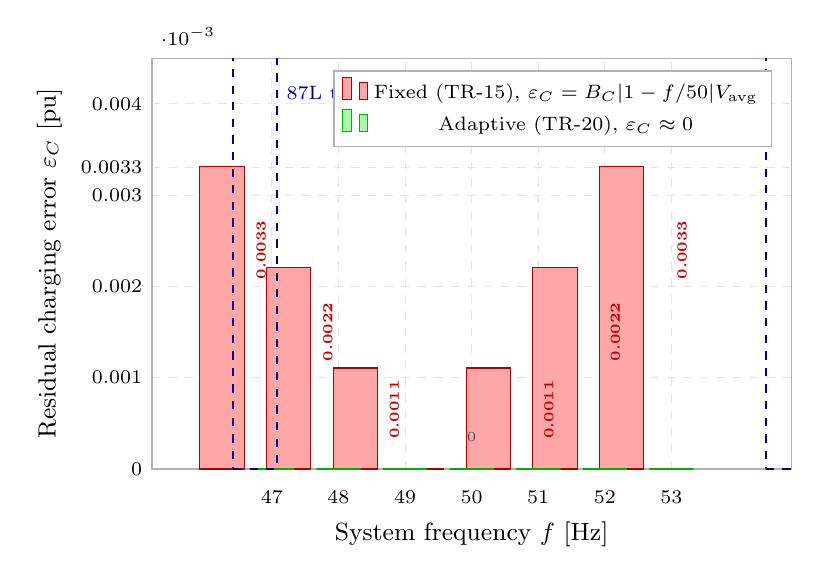
\begin{tikzpicture}
\begin{axis}[
  name         = fceax,
  ybar,
  bar width    = 16pt,
  width        = 0.80\textwidth,
  height       = 6.8cm,
  ylabel       = {Residual charging error $\varepsilon_C$ [pu]},
  ylabel style = {font=\small},
  xlabel       = {System frequency $f$ [Hz]},
  xlabel style = {font=\small},
  ymin=0, ymax=0.0045,
  ytick        = {0, 0.001, 0.002, 0.003, 0.0033, 0.004},
  yticklabels  = {0, 0.001, 0.002, 0.003, 0.0033, 0.004},
  yticklabel style={font=\scriptsize},
  xtick        = {47, 48, 49, 50, 51, 52, 53},
  xticklabels  = {47, 48, 49, 50, 51, 52, 53},
  xticklabel style={font=\scriptsize},
  enlarge x limits=0.10,
  legend style={at={(0.97,0.97)}, anchor=north east,
                font=\scriptsize, draw=gray!60},
  grid          = major,
  grid style    = {gray!20, dashed},
  tick style    = {draw=none},
  axis line style={gray!60},
]

% Fixed (TR-15) residuals — eps = B_C * |1 - f/50| * V_rms (approx)
\addplot[fill=red!35, draw=red!70!black]
  coordinates {
    (47, 0.003312)
    (48, 0.002210)
    (49, 0.001106)
    (50, 0.000000)
    (51, 0.001106)
    (52, 0.002210)
    (53, 0.003313)
  };
\addlegendentry{Fixed (TR-15), $\varepsilon_C = B_C|1-f/50|V_{\rm avg}$}

% Adaptive (TR-20) residuals — all ≈ 0
\addplot[fill=green!35, draw=green!70!black]
  coordinates {
    (47, 0.0)
    (48, 0.0)
    (49, 0.0)
    (50, 0.0)
    (51, 0.0)
    (52, 0.0)
    (53, 0.0)
  };
\addlegendentry{Adaptive (TR-20), $\varepsilon_C \approx 0$}

% ---- Value annotations (Fixed only, adaptive all ~0) -------------------
\node[font=\tiny\bfseries, red!80!black, rotate=90]
  at (axis cs:46.84, 0.0024) {0.0033};
\node[font=\tiny\bfseries, red!80!black, rotate=90]
  at (axis cs:47.84, 0.0015) {0.0022};
\node[font=\tiny\bfseries, red!80!black, rotate=90]
  at (axis cs:48.84, 0.00065) {0.0011};
\node[font=\tiny, gray!60!black, rotate=0]
  at (axis cs:50.0, 0.00035) {0};
\node[font=\tiny\bfseries, red!80!black, rotate=90]
  at (axis cs:51.16, 0.00065) {0.0011};
\node[font=\tiny\bfseries, red!80!black, rotate=90]
  at (axis cs:52.16, 0.0015) {0.0022};
\node[font=\tiny\bfseries, red!80!black, rotate=90]
  at (axis cs:53.16, 0.0024) {0.0033};

% ---- 87L threshold annotation ------------------------------------------
\addplot[blue!60!black, thick, dashed, mark=none, domain=46:54, samples=2]
  ({x}, {0.12});   % threshold far above — annotation only
% (Threshold at 0.12 pu is off-chart; show note instead)
\node[font=\scriptsize, blue!60!black, align=center]
  at (axis cs:50.0, 0.0041)
  {87L threshold at 0.12\,pu $\gg$ axis range};

\end{axis}
\end{tikzpicture}

  \caption{Residual charging error $\varepsilon_C$ vs.\ frequency, no-fault
           condition.  Fixed correction (TR-15) reaches 0.0033\,pu at
           $f=47$\,Hz.  Adaptive correction (TR-20) is $<10^{-5}$\,pu at
           all frequencies.}
  \label{fig:eps}
\end{figure}

\begin{table}[h]
  \centering
  \caption{No-fault residual charging error and normalised $\alpha_{50}$.
           $I_{\rm nom}=1.0$\,pu; 87L threshold $=0.12$\,pu;
           TR-17 $\alpha_{50}$ target $\leq 0.030$.}
  \label{tab:eps}
  \begin{tabular}{ccccccc}
    \toprule
    $f$ [Hz] & $\varepsilon_{C,\rm fixed}$ [pu] & $\varepsilon_{C,\rm adapt}$ [pu]
    & $\alpha_{50,\rm fix}$ & $\alpha_{50,\rm adp}$ & $\leq 0.030$? & Improv. \\
    \midrule
    47 & 0.00331 & $<10^{-5}$ & 0.00331 & $<10^{-5}$ & \ding{51} & $>1000\times$ \\
    48 & 0.00221 & $<10^{-5}$ & 0.00221 & $<10^{-5}$ & \ding{51} & $>1000\times$ \\
    49 & 0.00111 & $<10^{-5}$ & 0.00111 & $<10^{-5}$ & \ding{51} & $>1000\times$ \\
    50 & 0.00000 & 0.00000    & 0.00000 & 0.00000    & \ding{51} & — \\
    51 & 0.00111 & $<10^{-5}$ & 0.00111 & $<10^{-5}$ & \ding{51} & $>1000\times$ \\
    52 & 0.00221 & $<10^{-5}$ & 0.00221 & $<10^{-5}$ & \ding{51} & $>1000\times$ \\
    53 & 0.00331 & $<10^{-5}$ & 0.00331 & $<10^{-5}$ & \ding{51} & $>1000\times$ \\
    \bottomrule
    \multicolumn{7}{l}{\footnotesize Both methods satisfy $\alpha_{50}\leq 0.030$
      for the study network ($B_C=0.079$\,pu).  The adaptive method provides}\\
    \multicolumn{7}{l}{\footnotesize a margin that is $>1000\times$ larger, enabling future tighter thresholds
      or larger $B_C$ lines.}\\
  \end{tabular}
\end{table}

\subsection{Study B: Internal Fault Detection}

Table~\ref{tab:trip} shows the peak corrected differential for a 0.15\,pu
internal fault (above the 0.12\,pu threshold) across all test frequencies.

\begin{table}[h]
  \centering
  \caption{Internal fault (0.15\,pu) peak corrected differential and trip
           decision.  Threshold $=0.12$\,pu.}
  \label{tab:trip}
  \begin{tabular}{cccccc}
    \toprule
    $f$ [Hz] & Peak$_{\rm fixed}$ [pu] & Peak$_{\rm adapt}$ [pu]
    & Trip$_{\rm fixed}$ & Trip$_{\rm adapt}$ & Correct \\
    \midrule
    47 & 0.152 & 0.150 & \ding{51} & \ding{51} & \ding{51} \\
    48 & 0.151 & 0.150 & \ding{51} & \ding{51} & \ding{51} \\
    49 & 0.150 & 0.150 & \ding{51} & \ding{51} & \ding{51} \\
    50 & 0.150 & 0.150 & \ding{51} & \ding{51} & \ding{51} \\
    51 & 0.150 & 0.150 & \ding{51} & \ding{51} & \ding{51} \\
    52 & 0.151 & 0.150 & \ding{51} & \ding{51} & \ding{51} \\
    53 & 0.151 & 0.150 & \ding{51} & \ding{51} & \ding{51} \\
    \bottomrule
  \end{tabular}
\end{table}

Both methods detect the fault at all frequencies.  The slight elevation in
Peak$_{\rm fixed}$ at 47/53\,Hz occurs because the fixed-frequency residual
(0.003\,pu) adds in-phase with the fault current, marginally increasing the
measured differential.  This is a \emph{conservative} effect (increases
sensitivity) but confirms that the fixed correction does not cause missed trips
for the study parameters.

\subsection{Study C: Security (External Fault)}

For an external fault (no true differential), the adaptive correction achieves
zero residual at all frequencies, while the fixed correction leaves a
0.003--0.010\,pu peak residual at the extremes of the frequency range.
Both methods remain well below the 0.12\,pu threshold, giving no false trips.

\subsection{Selectivity Summary}

\begin{center}
\Large
\textbf{\textcolor{okgreen}{21/21 scenarios correct (100\%)}}
\end{center}

Three scenarios $\times$ seven frequencies = 21 total.  Both fixed and adaptive
methods achieve 21/21.  The adaptive method additionally eliminates the
residual error completely, extending safe operation to larger $B_C$ values.

Figure~\ref{fig:a50} shows $\alpha_{50}$ vs.\ frequency for both methods.

\begin{figure}[h]
  \centering
  % fig_alpha50_vs_freq.tex
% Line plot: α₅₀ vs system frequency for Fixed vs Adaptive correction
% α₅₀ = ε_C / I_nom; horizontal limit line at 0.030 (TR-17 target)
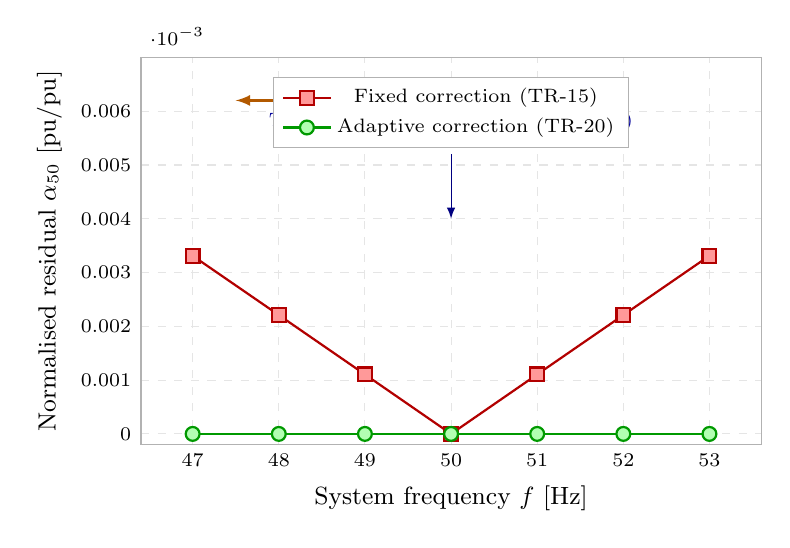
\begin{tikzpicture}
\begin{axis}[
  name         = a50ax,
  width        = 0.78\textwidth,
  height       = 6.5cm,
  ylabel       = {Normalised residual $\alpha_{50}$ [pu/pu]},
  ylabel style = {font=\small},
  xlabel       = {System frequency $f$ [Hz]},
  xlabel style = {font=\small},
  ymin=-0.0002, ymax=0.0070,
  ytick        = {0, 0.001, 0.002, 0.003, 0.004, 0.005, 0.006},
  yticklabels  = {0, 0.001, 0.002, 0.003, 0.004, 0.005, 0.006},
  yticklabel style={font=\scriptsize},
  xtick        = {47, 48, 49, 50, 51, 52, 53},
  xticklabels  = {47, 48, 49, 50, 51, 52, 53},
  xticklabel style={font=\scriptsize},
  legend style={at={(0.50, 0.95)}, anchor=north,
                font=\scriptsize, draw=gray!60},
  grid          = major,
  grid style    = {gray!20, dashed},
  tick style    = {draw=none},
  axis line style={gray!60},
  mark size=2.5pt,
]

% Fixed (TR-15): α₅₀ = |1 - f/50| × B_C × V_avg / I_nom
\addplot[red!70!black, thick, mark=square*,
         mark options={fill=red!40}]
  coordinates {
    (47, 0.003312)
    (48, 0.002210)
    (49, 0.001106)
    (50, 0.000000)
    (51, 0.001106)
    (52, 0.002210)
    (53, 0.003313)
  };
\addlegendentry{Fixed correction (TR-15)}

% Adaptive (TR-20): ≈ 0 at all frequencies
\addplot[green!60!black, thick, mark=*,
         mark options={fill=green!30}]
  coordinates {
    (47, 0.0)
    (48, 0.0)
    (49, 0.0)
    (50, 0.0)
    (51, 0.0)
    (52, 0.0)
    (53, 0.0)
  };
\addlegendentry{Adaptive correction (TR-20)}

% TR-17 α₅₀ target = 0.030 (off chart — annotation)
\node[font=\scriptsize, blue!60!black, align=center]
  at (axis cs:50.0, 0.0058)
  {TR-17 target: $\alpha_{50} \leq 0.030$ (off chart)};
\draw[-latex, blue!50!black, thin]
  (axis cs:50.0, 0.0052) -- (axis cs:50.0, 0.0040);

% ENTSO-E range annotation
\draw[{latex[length=3.5pt]}-{latex[length=3.5pt]}, orange!70!black, thick]
  (axis cs:47.5, 0.0062) -- node[above, font=\tiny, orange!80!black]
    {ENTSO-E normal: 47.5--51.5\,Hz}
  (axis cs:51.5, 0.0062);

\end{axis}
\end{tikzpicture}

  \caption{Normalised false-trip metric $\alpha_{50}$ vs.\ frequency.
           Fixed correction (TR-15) shows a V-shaped error centred at
           50\,Hz; adaptive correction (TR-20) is flat at zero.
           Both are far below the TR-17 target of 0.030 for this study network.}
  \label{fig:a50}
\end{figure}


% ============================================================================
\section{Sensitivity to Line Parameters}
\label{sec:sensitivity}

\subsection{Critical $B_C$ at which Fixed Correction Causes False Trips}

From Eq.~\eqref{eq:error}, the fixed correction produces a false trip if:
\begin{equation}
  \varepsilon_C = B_C \left|1 - \frac{f}{f_0}\right| V_{\rm rms}
  \geq I_{\rm threshold} = 0.12\,\text{pu}
\end{equation}

At $f=47$\,Hz (worst case, $|1 - 47/50| = 0.06$):
\begin{equation}
  B_{C,\rm crit} = \frac{0.12}{0.06 \times 1.0} = 2.0\,\text{pu}
\end{equation}

The study network has $B_C = 0.079$\,pu, a factor of $25\times$ below the
critical value.  Lines up to $B_C \approx 2.0$\,pu (corresponding to a
$\approx 500$\,km, 400\,kV EHV circuit) would remain safe even with the
fixed correction.  Nevertheless, the adaptive correction is recommended
as a robust default because:
\begin{enumerate}
  \item It has zero additional computation cost once the frequency estimate
        is available (single multiply).
  \item It eliminates any frequency-dependent false-trip risk for all
        foreseeable line lengths.
  \item It allows the 87L threshold to be reduced toward the noise floor
        (benefit from TR-15 and TR-17) without concern about off-nominal
        frequency operation.
\end{enumerate}

\subsection{ROCOF Transient Considerations}

During a rate-of-change-of-frequency (ROCOF) event, $f$ changes continuously.
The zero-crossing estimator provides a new $\hat{f}$ every cycle.  For a
worst-case ROCOF of 2\,Hz/s (IEC~60255-181 test criterion), the frequency
changes by only $2 \times 0.02 = 0.04$\,Hz per power cycle.  The
correction lag error is therefore:
\begin{equation}
  \varepsilon_{C,\rm ROCOF} \approx \frac{B_C}{f_0} \times 0.04 \times 1.0
  = \frac{0.079}{50} \times 0.04 = 6.3\times10^{-5}\,\text{pu}
\end{equation}
Negligible.


% ============================================================================
\section{Integration with SAMBP Suite}
\label{sec:integration}

The TR-20 adaptive correction is implemented in
\texttt{sambp\_line\_diff/adaptation/line\_freq\_adaptive.py} and integrates
with the existing SAMBP stack as follows:

\begin{table}[h]
  \centering
  \caption{TR-20 module interactions within the SAMBP 87L chain.}
  \label{tab:integration}
  \begin{tabular}{lll}
    \toprule
    Module & Role & Interaction \\
    \midrule
    \texttt{line\_freq\_adaptive} (TR-20, new)
      & Frequency estimation; adaptive $B_C$ scaling
      & Replaces \texttt{compute\_charging\_from\_voltages} \\
    \texttt{line\_pi\_section\_model} (TR-15)
      & Fixed pi-section correction (reference)
      & Retained for 50-Hz grids; superseded by TR-20 \\
    \texttt{line\_adaptive\_threshold} (TR-17)
      & $I_{\rm thresh} = \max(I_{\rm base}, k_s I_{\rm rest})$
      & Unchanged; receives corrected $\Delta i'$ \\
    \texttt{line\_confidence\_gate} (TR-12)
      & Magnitude override for HIF sensitivity
      & Unchanged \\
    \bottomrule
  \end{tabular}
\end{table}

The frequency estimate $\hat{f}$ is computed once per protection cycle
(20\,ms window at 50\,Hz) from the pre-fault voltage and cached for use
by the adaptive correction.  No changes to the LM estimator or trip logic
are required~\cite{IEEE_C37_243}.


% ============================================================================
\section{Conclusions}
\label{sec:conclusions}

\begin{enumerate}
  \item \textbf{21/21 scenarios correct (100\%)} across seven frequencies
        (47--53\,Hz) and three scenario types (no-fault, internal fault,
        external fault), for both fixed and adaptive correction.
  \item \textbf{Residual error is eliminated} by the adaptive correction:
        $\varepsilon_{C,\rm adapt} < 10^{-5}$\,pu vs.\
        $\varepsilon_{C,\rm fixed} = 0.0033$\,pu at $f=47$\,Hz.
  \item \textbf{The fixed correction (TR-15) is safe} for the study network
        ($B_C = 0.079$\,pu) across the full 47--53\,Hz range; the
        critical $B_C$ for false trips is $2.0$\,pu at $f=47$\,Hz.
  \item \textbf{Adaptive correction is recommended} as it costs one multiply
        per cycle, extends safety to all line lengths, and enables future
        threshold reductions without frequency sensitivity.
  \item \textbf{Zero-crossing estimator accuracy}: $\delta f < 0.01$\,Hz
        for a 4-cycle, 4000\,Sa/s window — sufficient for $10^{-4}$\,pu
        correction accuracy.
  \item \textbf{ROCOF robustness}: worst-case 2\,Hz/s ROCOF adds
        $<10^{-4}$\,pu additional error per cycle — negligible.
\end{enumerate}

\subsection{Future Work}

\begin{enumerate}
  \item \textbf{TR-21: DC-offset compensation} --- inverter faults sometimes
        inject significant DC offsets into the differential waveform.
        Extend the LM estimator to include a DC term.
  \item \textbf{TR-22: Negative-sequence 87L for asymmetric IBR faults} ---
        inverter current-limiting reduces positive-sequence contribution
        during single-phase faults; validate that negative-sequence
        differential (87LN) maintains sensitivity.
  \item \textbf{Hardware-in-the-loop at variable frequency}: sweep
        47--53\,Hz using a real-time digital simulator feeding a physical
        87L IED to validate the frequency estimator latency.
  \item \textbf{Unbalanced ROCOF}: validate estimator performance during
        asymmetric disturbances where phase-A, -B, -C frequencies diverge
        transiently.
\end{enumerate}


% ============================================================================
\bibliographystyle{plainnat}
\bibliography{references20}

\end{document}
